\documentclass[a4paper]{article}
\usepackage[utf8]{inputenc}
\usepackage[francais]{babel}
\usepackage{hyperref}
\usepackage{entete}
\usepackage{noitemsep}
\usepackage{euscript} 
\usepackage{amsmath,amssymb,amsfonts,amsthm}
\usepackage{graphicx,graphics,epsfig,subfigure,color}
\usepackage{url}
%\usepackage{algorithm2e}
\usepackage{multicol}
\usepackage{a4wide}
\usepackage{latexsym}
\usepackage{verbatim}
\setlength{\textheight}{23.6cm}
\setlength{\topmargin}{-1cm}
\setlength{\textwidth}{165mm}
\setlength{\oddsidemargin}{1.5mm}

\usepackage{pdfpages}
%\renewcommand{\baselinestretch}{0.85}

\pagenumbering{gobble}  %% remove page number

%\input{macroAlgo}
%\dontprintsemicolon

\setlength{\parindent}{0pt}  %%suppression indentation

\newif\ifcorrection
\correctiontrue   %% With correction
\correctionfalse   %% Reviewer's version


\begin{document}
\selectlanguage{francais}
\author{D. Fourer, L. Lagon}
\newcommand{\universityname}{IUT d'\'Evry Val d'Essonne}
\newcommand{\deptname}{D\'epartement TC (S3)}
\newcommand{\years}{2023-2024}

%------------------- TITRE -----------------------------------------
\date{Septembre 2021} 
\TDHead{\universityname}{\deptname}{R3.07, \years}{\large TD : Fonction affines}
%\TDHead{DUT TC}{}{\large TIC3: Fonctions avanc\'ees d'un tableur}
%-------------------------------------------------------------------


\exost Prise en main d'une fonction affine :


A partir du \href{https://www.geogebra.org/m/TGuBC7JW}{lien} suivant, définir : 

\begin{enumerate}
    \item Interpréter de manière graphique les coefficients $a$ et $b$
    \item Comment se calculent les coefficients $a$ et $b$
    \item Soient A, B deux points appartenant à la droite représentative d’une fonction affine $f$. Définir cette fonction algébriquement à l’aide des coordonnées des deux points.
\end{enumerate}

\vspace{0.5cm}
\exost Passer de la forme graphique à la forme algébrique


Soient 3 fonctions $f$,$g$ et $h$ passant respectivement par les points A,B,C,D,E et F de $\mathbb{R}^2$. Définir ces 3 fonctions algébriquement.
\begin{figure}[!h]
    \centering
    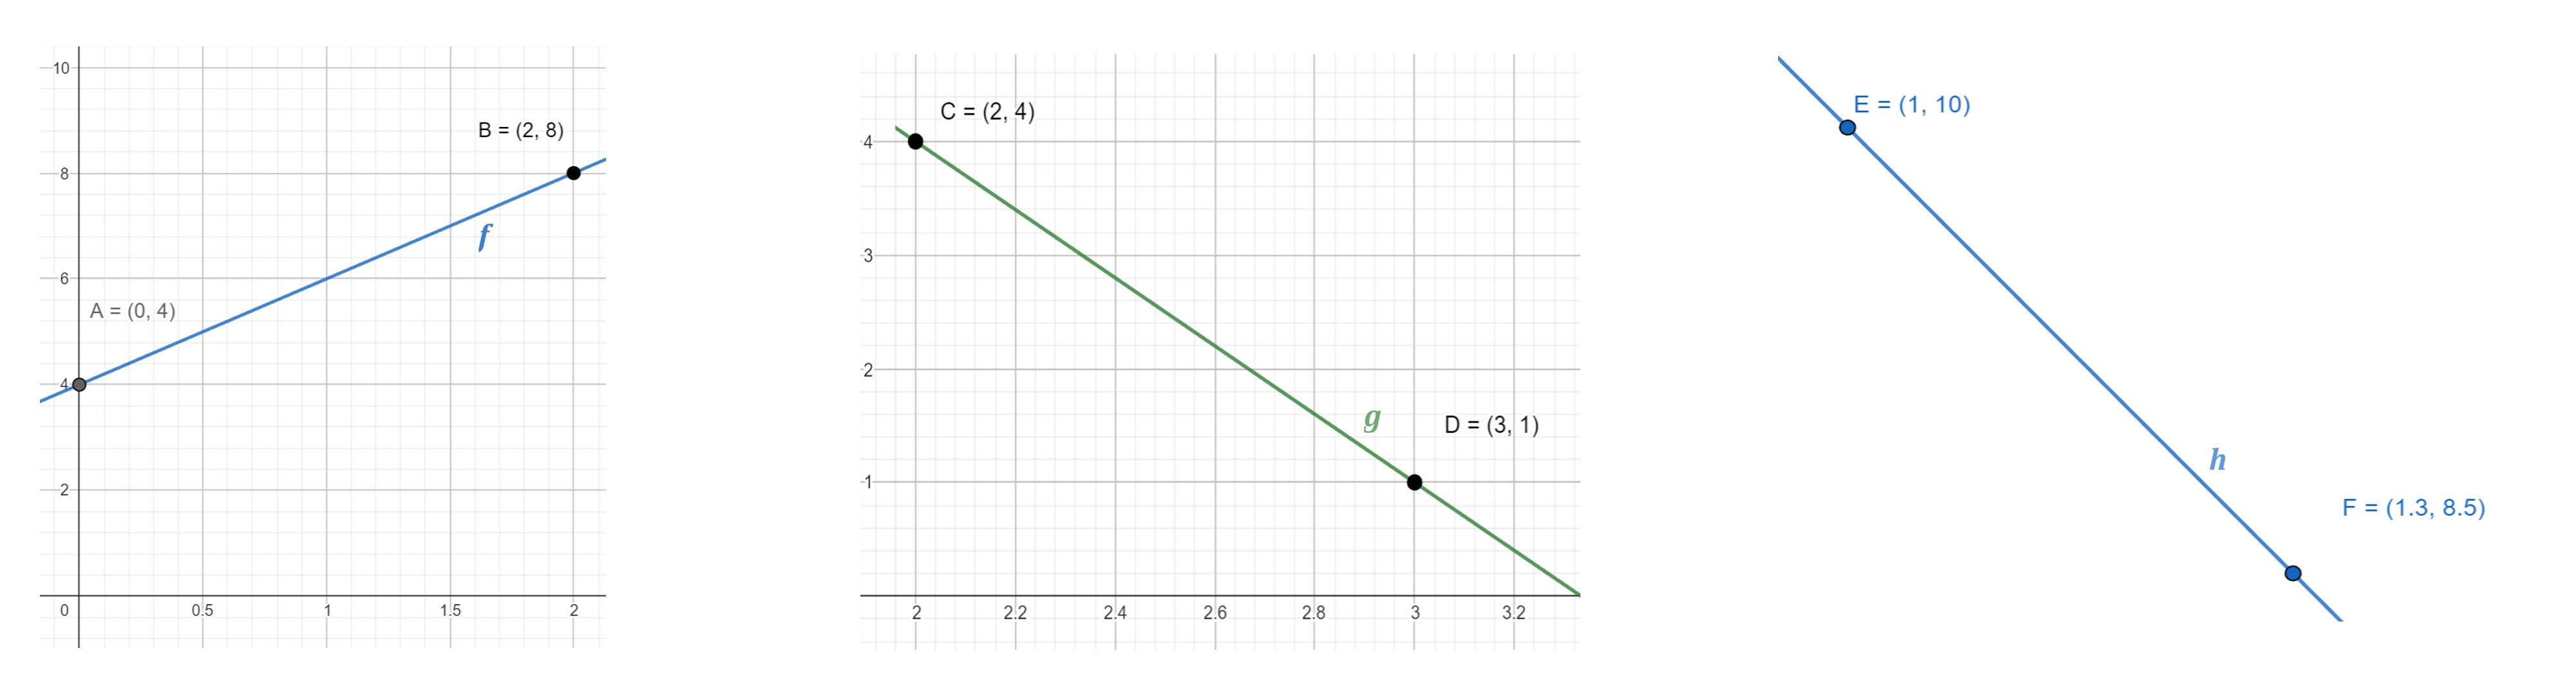
\includegraphics[width=1\linewidth]{aff.jpg}
    \caption{Les fonctions $f,g$ et $h$}
    \label{fig:enter-label}
\end{figure}



\vspace{0.5cm}
\exost L'impot sur le revenu

On cherche à modéliser l’impôt sur le revenu en fonction des revenus d’une personne à partir des données suivantes 
\begin{figure}[!h]
    \centering
    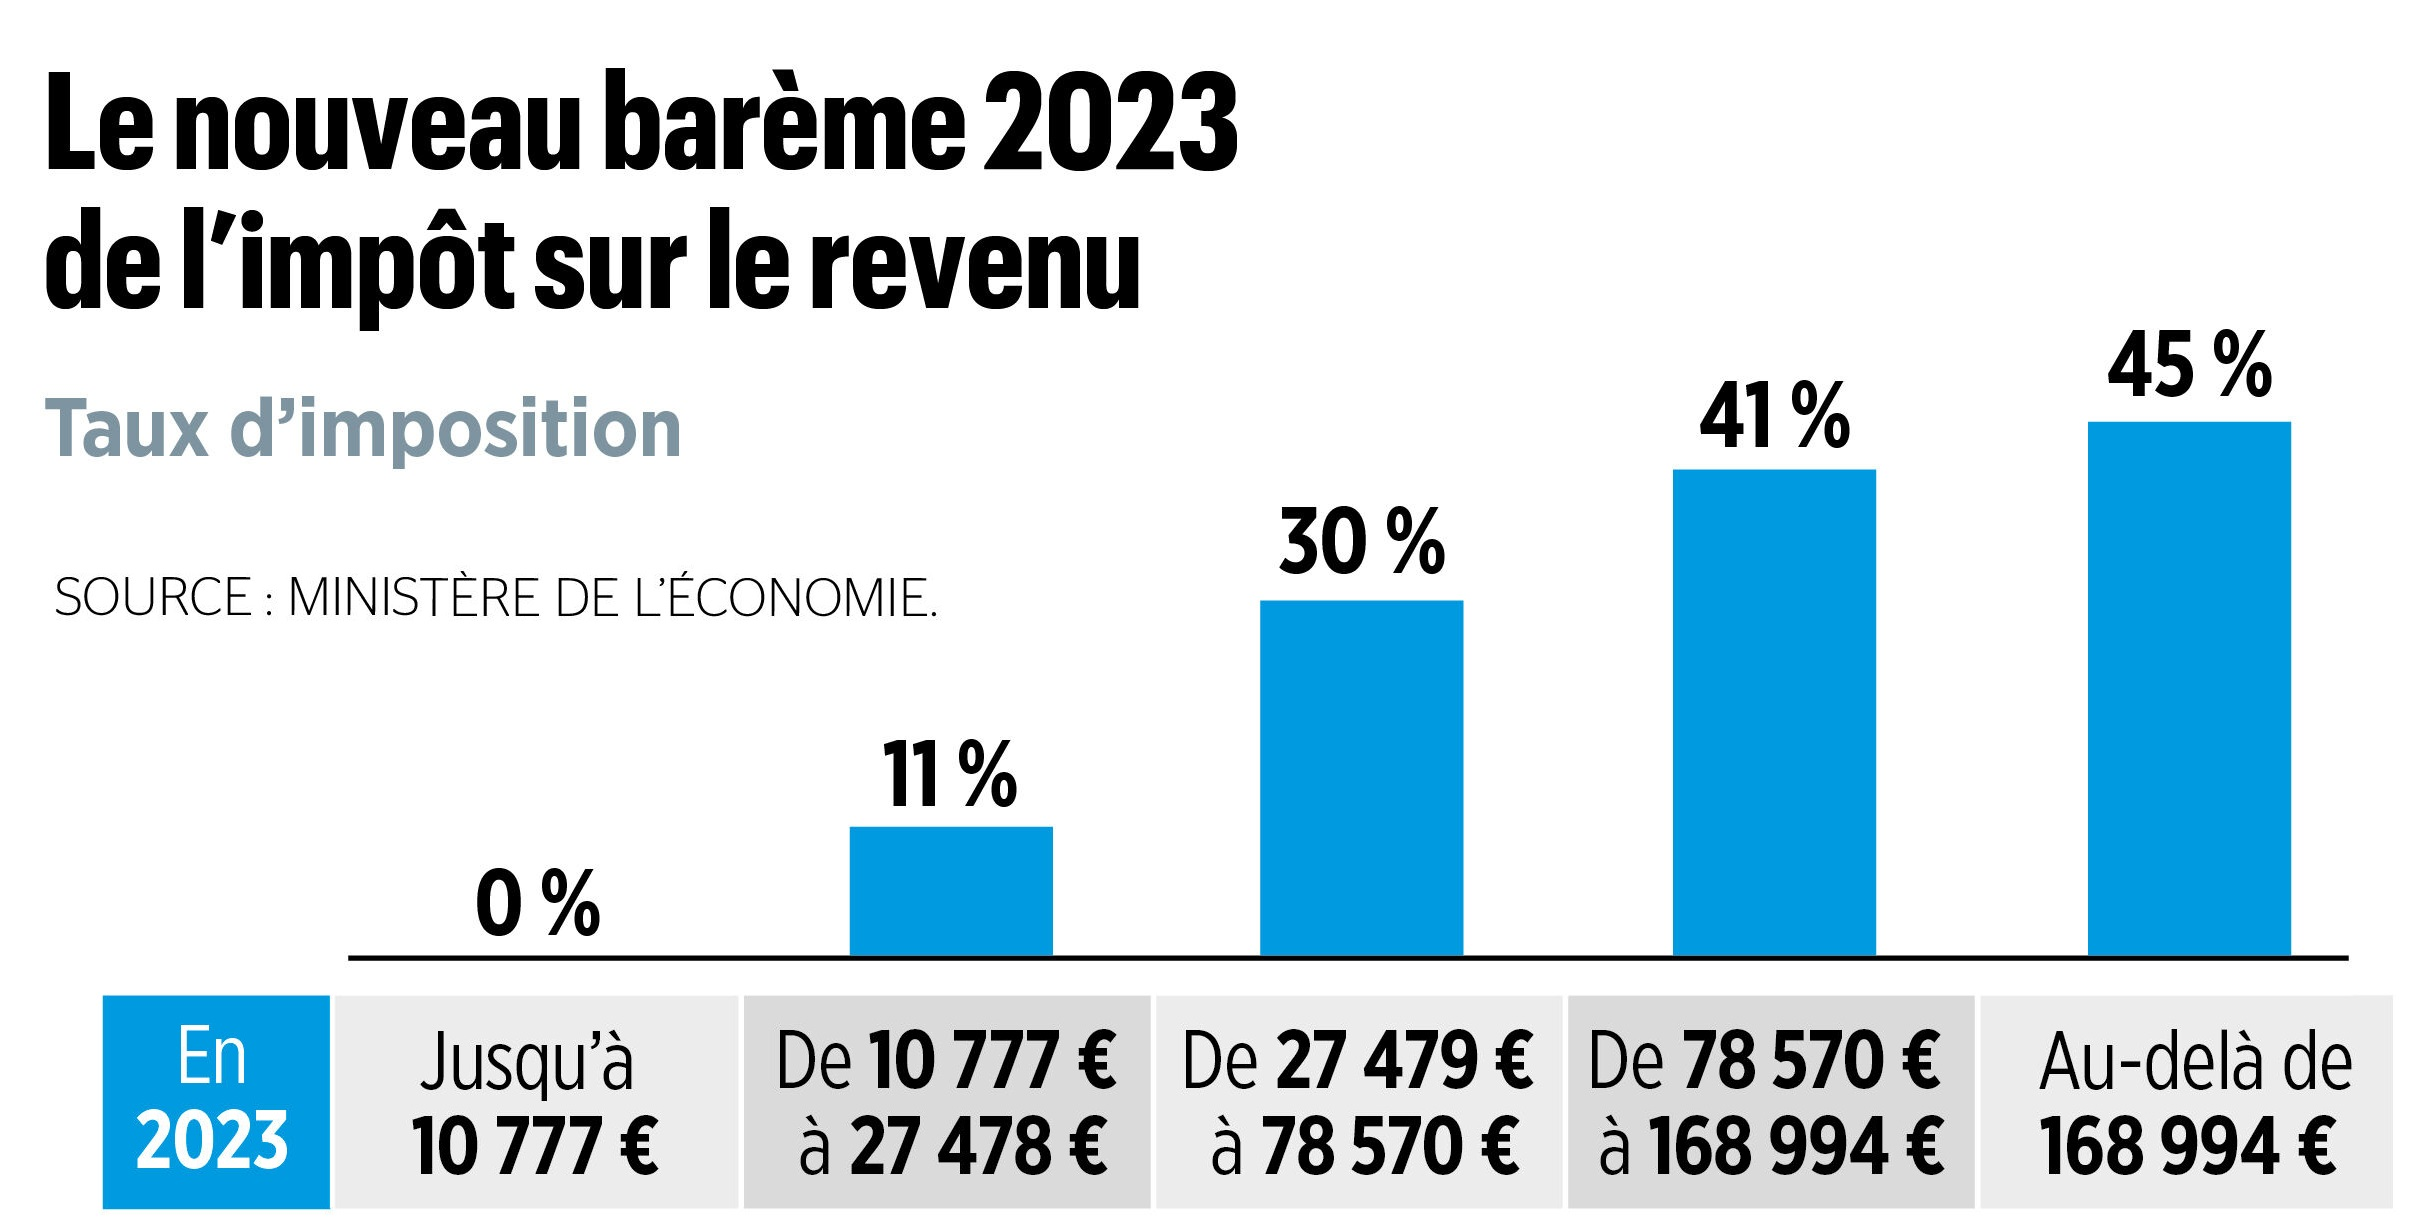
\includegraphics[width=0.5\linewidth]{impot.jpg}
    \caption{Calcul de l'impot sur le revenu}
    \label{fig:enter-label}
\end{figure}
\begin{enumerate}
    \item Combien doit payer une personne ayant 20 000€ de revenus annuels ?
    \item Combien doit payer une personne ayant 50 000€ de revenus annuels ?
    \item Modéliser l’impôt sur le revenu en fonction des revenus d’une personne à l’aide de 5 fonctions affines
\end{enumerate}



\vspace{0.5cm}
\exost Approximation affine d'un polynôme

Donner l’approximation affine de la fonction du second degré $f(x)=4x²+2x+3$ \ $\forall x \in [3;5]$

\vspace{0.5cm}
\exost Quadrature du cercle en 4 morceaux

Soit $x,y \in [0;1]$ et $\mathbb{C}$, un cercle  de rayon 1. On suppose un point $M$ de coordonnées $M(x,y) \in \mathbb{C}$. 
\begin{enumerate}
    \item Trouver une condition liant x et y
%x²+y²=1
    \item Exprimer y en fonction de x
%y=Racine(1-x²)
    \item A partir de la relation obtenue, réaliser une approximation affine en 4 morceaux du quart de cercle

\begin{figure}[!h]
    \centering
    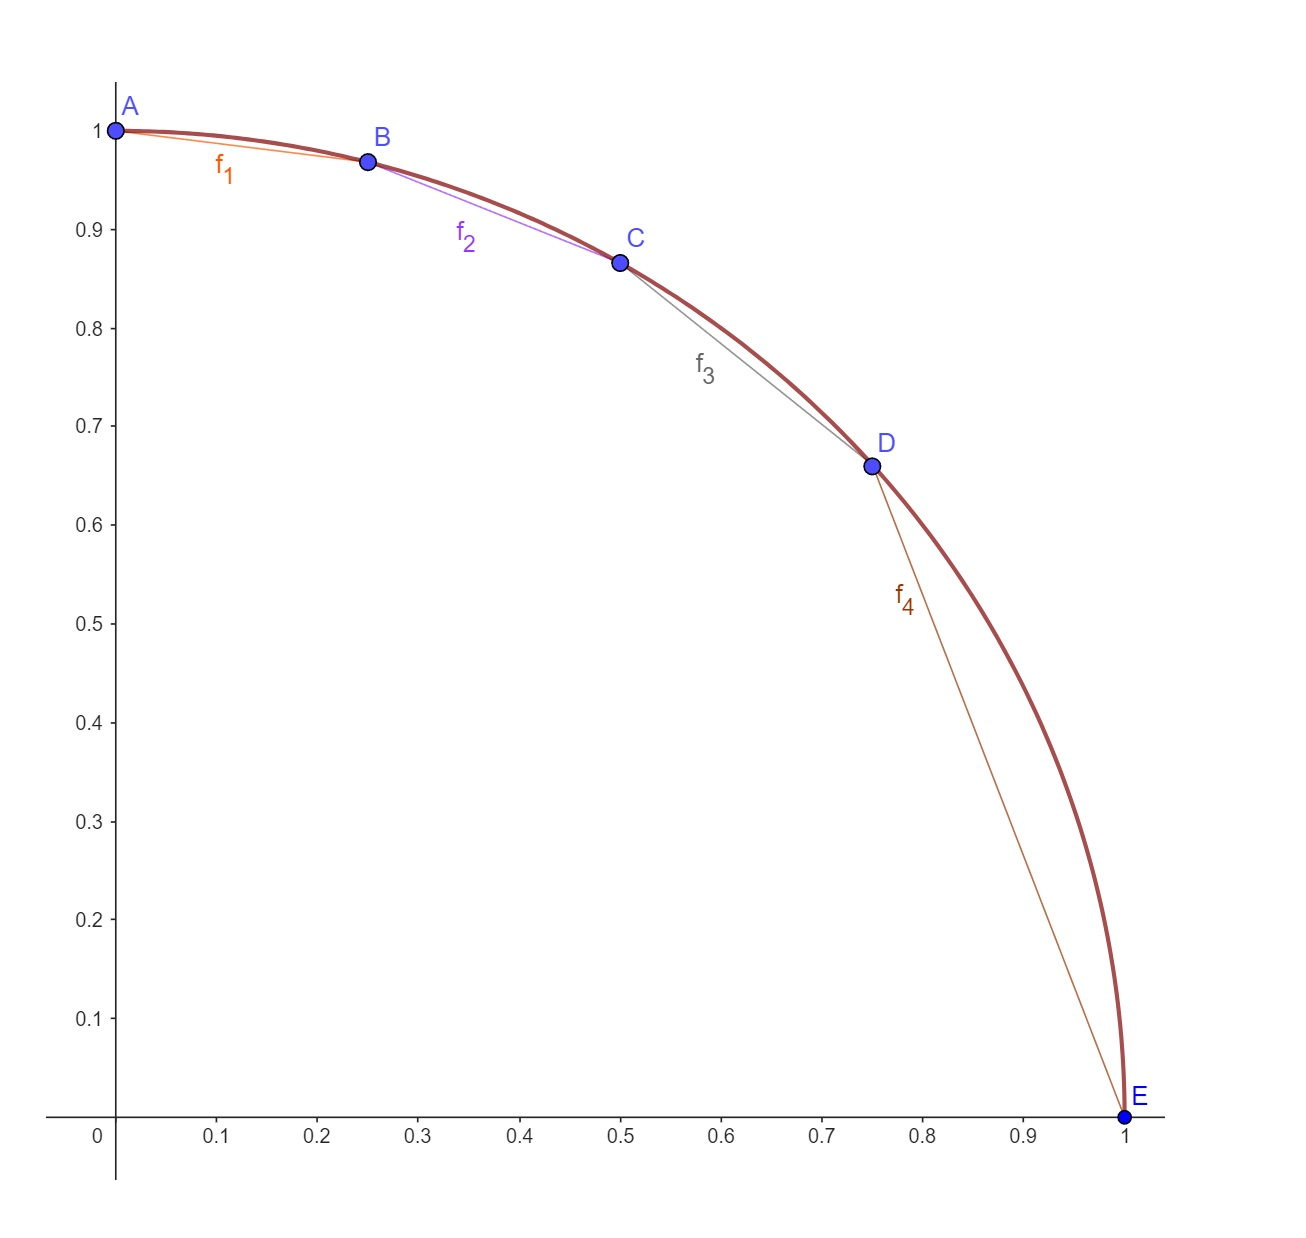
\includegraphics[width=0.5\linewidth]{cercle.jpg}
    \caption{Cercle de rayon 1}
    \label{fig:enter-label}
\end{figure}


%On définit A(0;1) B(1/4;racine(15)/4) C(1/2;racine(3)/2) D(3/4;racine(7)/4  E(1;0) 
%On cherche f1(x); f2(x), f3(x) et f4(x)
%a1 = racine (15)-4       b1 = 1
%a2 = 2racine(3)-racine(15)   b2 = (racine(15)-racine(3))/2
%a3 = racine(7) - 2 racine(3)      b3 = 1/2 * 3racine(3) - racine(7)
%a4 = -racine(7)  b4 = racine(7)

    \end{enumerate}


\end{document}

% End Of File

